% -*- root: ../main.tex -*-

% Esporre l'obiettivo del progetto dandone una visione complessiva. Devono essere illustrate le caratteristiche salienti del progetto; deve essere chiara la distinzione tra le tecnologie usate/assemblate durante lo svolgimento dell'elaborato e il contributo tecnologico/scientifico e effettivamente apportato dal gruppo.
% 3000 - 6000 battute

\chapter{Introduzione}
Smart DogHouse è un progetto che nasce con l'intento di migliorare le condizioni dei cani che si trovano ospiti di un \textbf{canile}, mediante l'introduzione di un \textbf{supporto informatico} che possa, da un lato, \textbf{facilitare operazioni} che già prima venivano svolte e dall'altro \textbf{introdurre nuovi strumenti} che vadano a migliorare la gestione del canile.

\section{Overview}
Come riferimento è stato preso in considerazione il \textbf{ canile comunale di Pisa}, il quale gestore si è offerto di indirizzarci permettendoci di rivolgerci a lui per avere feedback e indicazioni basate su \textbf{esperienze reali}. 

L'idea ha avuto origine dopo un colloquio con il gestore del canile che, raccontando la propria esperienza, ha evidenziato alcuni \textbf{problemi} che riscontra nello svolgimento del proprio lavoro, molti dei quali sono risolvibili attraverso gli \textbf{strumenti} e le \textbf{competenze} che abbiamo a disposizione.
Successivamente, le informazioni ottenute dal canile di Pisa sono state confrontate e integrate a fronte di un colloquio con il \textbf{canile Comunale di Cesena}, la quale consulenza è stata indispensabile per riuscire a discernere gli \textbf{aspetti comuni }alla maggior parte dei canili da quelle che invece sono \textbf{peculiarità} di un canile specifico. 
Le domande e le risposte di entrambi i canili sono rese disponibili nel \href{https://github.com/SmartDogHouse/SmartDogHouse-Report/tree/main/Extra/Domande_Canile.pdf}{pdf relativo negli extra}.
Questa capacità di \textbf{astrazione} ci ha permesso di definire meglio gli \textbf{obiettivi}. 
Anche se questo non può essere considerato un progetto su commissione, abbiamo fede nel fatto che una volta sviluppata la nostra soluzione, essa possa essere utilizzata come base per sviluppare altri sistemi o rendere più tecnologici canili e gattili che riscontrano le stesse difficoltà.

        %CANILI
        \begin{figure}[H]
            \caption{I due canili interpellati in qualità di \textbf{esperti del dominio}}
            \label{fig:Canili}
            \centering
            
\includegraphics[width=0.8\textwidth]{Images/canili.png}
        \end{figure}

\section{Problemi}
Il canile di Pisa ospita circa una \textbf{sessantina} di cani e gatti di diversa \textbf{taglia}, \textbf{randagi} o \textbf{abbandonati}, che vengono prelevati dagli addetti del canile su segnalazione dei cittadini. I cani restano poi in cura finché non vengono \textbf{adottati}, mentre i gatti vengono \textbf{rilasciati} subito dopo aver ricevuto le cure  mediche ed essersi ripresi. Ad occuparsi della salute dei cani è un \textbf{responsabile sanitario} sempre presente nella struttura, che coordina alcuni \textbf{veterinari} convenzionati con la struttura. La situazione al canile di Cesena è similare, con la differenza che quest'ultimo non si occupa più del recupero di gatti randagi e il responsabile sanitario non coordina altri veterinari ma si occupa \textbf{in autonomia} di tutto ciò che riguarda la salute del cane, dai problemi di routine alle \textbf{operazioni chirurgiche}.

I principali problemi che vengono attualmente riscontrati sono i seguenti:
\begin{itemize}
    \item \textbf{responsabile sanitario:} il responsabile sanitario e alcuni veterinari convenzionati, risiedono all'interno del canile.
    Attualmente non è possibile monitorare in maniera continuativa lo stato di salute di un animale. Questo spesso si traduce in un intervento tardivo che porta con sé delle limitazioni che con una diagnosi più veloce si sarebbero potute evitare.
    \item \textbf{Rifornimento e consumi di cibo ed acqua:} in entrambi i canili la maggior parte del lavoro manuale viene svolta dai volontari che prestano attività in forma gratuita e fortemente discontinua. Non è possibile sapere a priori quanti volontari si presenteranno a dare una mano, ed essendo in tanti non è nemmeno possibile sapere chi ha svolto quali mansioni. Operazioni come il rifornimento di cibo ed acqua vanno quindi monitorate personalmente dal gestore che deve recarsi fisicamente nelle gabbie per controllare gli approvvigionamenti; inoltre non è nemmeno possibile conoscere la quantità di cibo ed acqua consumata da un cane, il che rende più difficile individuare i segnali alimentari che sono sintomi di alcuni problemi di salute.
    \item \textbf{Sorveglianza:} né il canile di Pisa, né quello di Cesena, attualmente, dispongono di un sistema di sorveglianza da remoto, pertanto nel momento in cui si verificano furti, effrazioni ed atti vandalici, non è possibile risalire agevolmente al colpevole. E' assente anche un sistema che possa permettere di sorvegliare da remoto cani che hanno particolari problemi. Nel caso di una gravidanza che volge al termine, ad esempio, il personale del canile è costretto a recarsi frequentemente sul luogo, durante la notte, per controllare se ha avuto inizio il travaglio o se si stanno verificando delle complicanze. Questa necessità crea un disagio al personale che si trova a doversi recare in canile fuori dall'orario di lavoro.
    
    \item \textbf{Assenza di supporto informatico}: attualmente nessuno dei due canili dispone di un'infrastruttura informatica già presente, da poter integrare; inoltre non dispongono nemmeno di un gestionale che dia supporto nella catalogazione degli animali presi in cura.
\end{itemize}
 




\section{Obiettivi}
L'obiettivo è quello di rendere il canile più "Smart", introducendo della strumentazione che permetta di risolvere in maniera parziale o totale le problematiche descritte precedentemente, mantenendo un costo accessibile. 

    \begin{figure}[H]
        \caption{Obbiettivi principali}
        \label{fig:Obbiettivi}
        \centering
       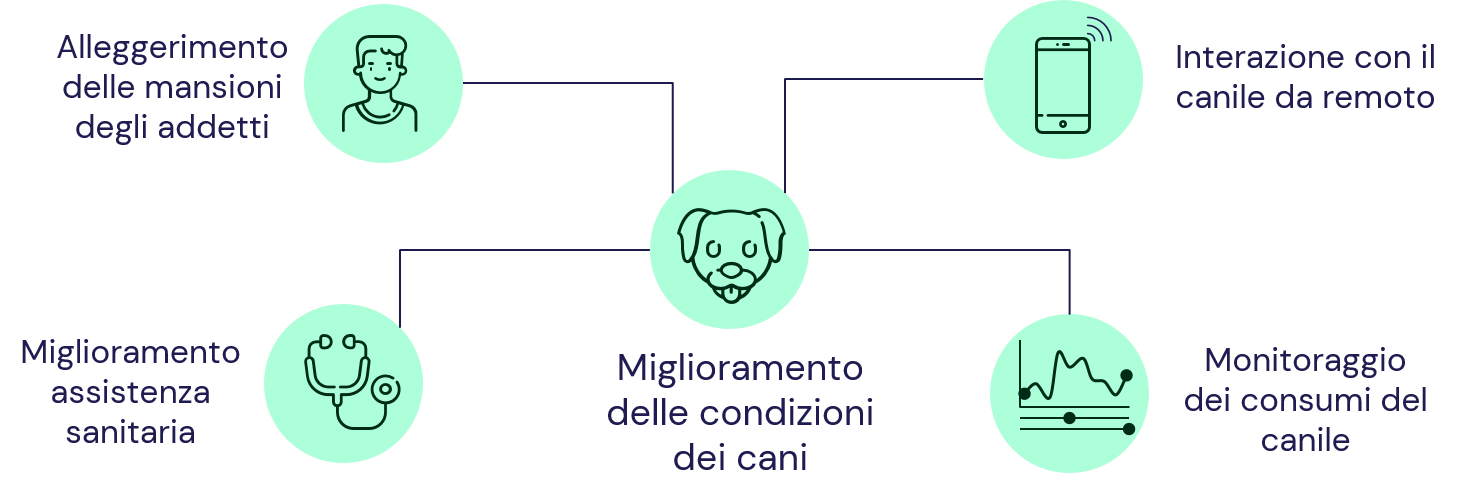
\includegraphics[width=1\textwidth]{Images/cani.png}
    \end{figure}
Nello specifico si vogliono incontrare le esigenze del gestore e degli addetti, agevolando le operazioni di:
\begin{itemize}
    \item \textbf{monitoraggio dello stato di salute dei cani} tramite:
    \begin{itemize}
        \item rilevazione dei \textbf{consumi} di cibo e acqua;
        \item monitoraggio del \textbf{comportamento} del cane.
    \end{itemize}
    In questo modo è possibile cogliere in maniera preventiva segnali che possono indicare un problema di salute e aiutare il \textbf{responsabile sanitario} nella risoluzione e nella diagnosi dello stesso. 
    \item automatizzazione delle operazioni di
\textbf{cura quotidiana} attraverso:
    \begin{itemize}
        \item automatizzazione del \textbf{rifornimento} di cibo e acqua
        \item possibilità di scegliere, per ciascun cane, la \textbf{quantità} del cibo da somministrare e la \textbf{frequenza}.
    \end{itemize}
    In questo modo è possibile gestire in maniera più precisa l'alimentazione dei cani e impostare delle quantità di cibo particolari in caso di condizioni di salute che richiedono un particolare piano alimentare, sollevando da questo incarico i volontari, che svolgono un'attività non tracciabile e discontinua. Inoltre, sarà possibile per il \textbf{responsabile sanitario} consultare i dati riguardanti l'alimentazione del cane e, di conseguenza, fornire diagnosi più precise. 
    \item \textbf{sorveglianza
globale del canile da remoto}: l'introduzione di un sistema di sorveglianza permetterà a chi di competenza di monitorare lo stato del canile anche da casa.
\item \textbf{Mantenimento dello storico dei dati registrati}: in questo modo sarà possibile consultare sia le informazioni riguardanti i cani che i dati che riguardano le condizioni del canile, permettendo anche di fare dei confronti su base temporale;
\item \textbf{consultazione dei dati acquisiti ed elaborati:} verrà fornita la possibilità di accedere allo storico dei dati medici su un Database, affinché il veterinario abbia una visione globale del quadro medico e possa velocemente filtrare le informazioni anche se non ha seguito il paziente dall'inizio. 
\item \emph{{[}optional{]}} 
\textbf{monitoraggio approfondito dei parametri vitali}: mediante l'installazione di sensoristica che permetta il monitoraggio di temperatura, battiti, movimento, ecc\ldots{} sarà possibile tenere ulteriormente sott'occhio cani che si trovano in condizioni di salute che necessitano di particolari attenzioni.

\item \textbf{Introduzione di un sistema informatico: } poiché non vi è un sistema informatico preesistente da integrare e vi sono poche disponibilità economiche, si è pensato di avvalersi di una piattaforma cloud sulla quale è possibile mantenere lo storico ed operare tramite l'utilizzo di un broker MQTT per la comunicazione  con sensori e attuatori. Questa soluzione è stata indicata come preferibile dal canile che ritiene più accessibile pagare mensilmente un servizio piuttosto che investire in una soluzione ad hoc. 

\end{itemize}





